\documentclass[lang=cn, 10pt, titlestyle=hang, oneside]{elegantbook}
\usepackage{graphicx}
\usepackage{subfigure}
\usepackage{pgfplots}
\pgfplotsset{compat=1.18}
\usepackage{multicol}
\renewcommand{\theequation}{\Roman{equation}}
\tcbuselibrary{skins}
\usepackage{xcolor}
\usepackage{enumitem} % 提供 inline 列表

\usepackage{etoolbox}
\title{九年级数学讲义(人教版)}





%%%%%%%%%%%%%%%%%%%%%%%%%%%%%%%%%%%%%%%%%%%%%%%%%%%%%%%%%%%%%%%%%%%%%%%%%%%%%%%%%%%%%
\begin{document}

\tableofcontents

\chapter{一元二次方程}



\begin{introduction}[本章学习目标]

\item 将一元二次方程整理为一般形式
\item 判定一元二次方程
\item 熟练掌握配方法
\item 使用配方法求最值
\item 用不同方式解一元二次方程

\end{introduction}

经过本章的学习,你至少需要掌握以上的内容,在完成学习后你可以根据习题的情况,对照上面的学习目标,检验自己的学习成果.

\section{一元二次方程基本}
\subsection{一元二次方程的定义}


\begin{definition}[课本P3第一段第三行]
  
等号两边都是整式,只含一个未知数,并且未知数的最高次数是2的方程,叫做一元二次方程. 以下是一元二次方程的一般形式:

\begin{equation}
    ax^2 + bx + c = 0 \ (a \neq 0)
    \label{general_formula}
\end{equation}

 
\end{definition}



根据课本的定义,要构成一个一元二次方程必须具有三个条件:
\begin{enumerate}
    \item 是整式方程
    \item 只含有一个未知数
    \item 未知数的最高次数为2
\end{enumerate}
\par
当三个条件同时满足时,该方程是一元二次方程.\\
\begin{remark}
    \(a\ne 0\)保证了该方程中含有未知数最高次数为2. 如果没有\(a\ne 0\),则该方程不一定为一元二次方程,如果\(a= 0\),则该方程是一个一元一次方程. 在做任何关于一元二次方程的题目时都得考虑一元二次方程的条件是否成立,尤其是注意看\(a\)的取值情况.
\end{remark}
\par
我们将\eqref{general_formula}中的$ax^2$称为二次项(未知数的次数为2),a是二次项的系数;$bx$称为一次项(未知数的次数为1),$b$是一次项系数;$c$称为常数项.
\par
%结构命名例题
\begin{example}
    分别写出下列方程的二次项系数、一次项系数和常数项
    \begin{enumerate}
        \item \( 6x^2+10x-5=0 \)
        \item \( 4x^2-4=0 \)
        \item \( 5x^2-21x+4=0 \)
    \end{enumerate}
\end{example}
\par
\begin{solution}
    分析:阅读题目,要求写出各列方程的二次项系数、一次项系数和常数项,注意系数和常数项的符号不能忽略.解答如下:
    \begin{enumerate}
        \item  二次项系数:\(6x^2\),一次项系数:\(10x\),常数项:\(-5\)
        \item  二次项系数:\(4x^2\),一次项系数:\(0\),常数项:\(-4\)
        \item  二次项系数:\(5x^2\),一次项系数:\(-21\),常数项:\(4\)
    \end{enumerate}
\end{solution}
$x$的值就是这个一元二次方程的解,也可以称作这个一元二次方程的根.
\begin{remark}
    在做题时,有时会把$x$的值称做方程的解,有时称作方程的根,其实这都是一个意思.
\end{remark}



%%%%%%%%%%%%%%%%%%%%%%%%%%%%%%%%%%%%%%%%%%%%%%%%%%%%%%%%%%%%%%%%%%%%%%%%%%%%%%
\subsection{一元二次方程一般式转化}

在解题时,我们通常会先将一元二次方程整理为一般形式($
ax^2 + bx + c = 0 \ (a \neq 0)
$)
\par




整理过程分两步:
\begin{enumerate}
    \item 移项、合并
    \item 将二次项的系数化为正数
\end{enumerate}
%整理-例题
\begin{example}
    把方程\((-x+2)(x-3)=2x-6\)化为一般形式,并写出它的二次项、一次项系数和常数项
\end{example}
\par
\begin{solution}
    分析:阅读题目,首先回忆整理一元二次方程的步骤,先方程化简,再看化简结果中的二次项系数是否为负,如果是,方程两边同时乘\(-1\)将二次项系数化为正数,最后根据结果写出它的二次项、一次项系数和常数项.解答如下:
    \begin{align*}
    (-x) \cdot x + (-x) \cdot (-3) + 2 \cdot x + 2 \cdot (-3)&=2x-6 \\
        -x^2 + 5x - 6 &= 2x - 6 \\
        -x^2 + 5x - 6 - 2x + 6 &= 0 \\
        -x^2 + 3x &= 0\\
         x^2 - 3x &= 0% \quad (\text{两边同乘以}-1)
    \end{align*}
    \begin{itemize}[label=]
        \item 二次项:$x^2$
        \item 一次项系数:$-3$
        \item 常数项:$0$
    \end{itemize}
\end{solution}
%%%%%%%%%%%%%%%%%%%%%%%%%%%%%%%%%%%练习1.1%%%%%%%%%%%%%%%%%%%%%%%%
\begin{exercise}
\small
    \setlength{\parindent}{0pt} % 取消段落缩进
    \setlength{\columnseprule}{0.01pt}
    \begin{multicols}{2}
        \begin{minipage}{1\linewidth}
        (1)将方程 $(3x-1)(x+2) = 2(x+1)$ 化为一般形式.
        \end{minipage}
        
        \begin{minipage}{1\linewidth}
        (2)将方程 $\dfrac{x}{3} - \dfrac{2x-1}{6} = \dfrac{x^2-4}{2}$ 化为一般形式,并写出各项系数.
        \end{minipage}

        \begin{minipage}{1\linewidth}
        (3)已知方程 $(x^2-9)(x+2) = (x-3)^3 + k$ 的常数项为0,求k的值.
        \end{minipage}

        \begin{minipage}{1\linewidth}
        (4)关于$x$的一元二次方程\(2(x-1)^2+b(x-1)+c=0\)化为一般形式后为\(2x^2-3x-1=0\),求\(b,c\)的值.
        \end{minipage}
        
    \end{multicols}
\end{exercise}


\subsection{判定一元二次方程}
在前面我们学习了一元二次方程的定义,如何将一元二次方程整理为一般形式.
先回顾前面一元二次方程定义:
\begin{enumerate}
    \item 是整式方程
    \item 只含有一个未知数
    \item 未知数的最高次数为2
\end{enumerate}
\par
构成一个一元二次方程必须具有这三个条件,当三个条件同时满足,可以判定一个方程是一元二次方程. 
\begin{remark}
没有整理好的方程要先整理,做相关题目时注意二次项的系数不能为0\((a\ne0)\).
\end{remark}
%%%%%%%%%%%%%%%%%%%%%%%%%%%%%%%%%%%%%%%%%%%%%%%%%%%%%%%%%%%%%%%%%%%%%%%%%%%%%%%%%%%%%%%%%%%%%%%%
%判定例题1
\begin{example}
    下列关于 \( x \) 的方程中,一定是一元二次方程的为({\hspace{3.5em}}).
    \begin{enumerate}[label=\Alph*.]
        \item \( x^2 + 2xy + y^2 = 0 \)
        \item \( x^2 - 2x + 3 = 0 \)
        \item \( x^2 - \frac{1}{x} = 0 \)
        \item \( ax^2 + bx + c = 0 \)
    \end{enumerate}
\end{example}
\par
\begin{solution}
    分析:阅读题目,要我们选出一定是一元二次方程的方程,需要结合一元二次方程的定义来解题,先整理方程,再看每个选项是否符合一元二次方程必须具有的三个条件.(由于本例题所有选项都整理过,所以步骤中跳过)解答如下:
    \begin{enumerate}[label=\Alph*.]
        \item 是整式方程,未知数的最高次数为2,但含有两个未知数(\(x,y\)),所以错误.
        \item 是整式方程,只含有一个未知数,未知数的最高次数为2,满足所有条件所以正确.选择B.
        \item 未知数的最高次数为2,只含有一个未知数,但是是分式方程,所以错误.
        \item 是整式方程,只含一个未知数,未知数的最高次数为2,但是a的取值无法确定,当\(a=0\)时,方程中的未知数的最高次数为1,不一定是一元二次方程,因为题目要求“一定是”,所以错误.
    \end{enumerate}
\end{solution}
%判定例题2
\begin{example}
关于$x$的方程 $(m^2 - 4)x^2 + (m - 2)x + 3 = 0$,当$m$ \underline{\hspace{3.5em}} 时,该方程是一元二次方程,当$m$ \underline{\hspace{3.5em}} 时,该方程是一元一次方程.
\end{example}
\par
\begin{solution}
    分析:阅读题目,先判断何时为一元二次方程. 这个方程中只需要确定$(m^2 - 4)$不等于0即可使方程是二元一次方程,所以列不等式$(m^2 - 4)\ne0$确定取值范围,然后填空. 再判断何时为一元一次方程,需要列$(m^2 - 4)=0$消除二次项使方程符合未知数最高次数为1的条件,还需要使一次项系数不等于0,由此列$(m-2)\ne 0$,最后综合答案填空,解答如下:
    
    一元二次方程条件:
    \[
    m^2 - 4 \neq 0 \Rightarrow m \neq \pm 2
    \]
    
    一元一次方程条件:
    \[
    \begin{cases}
    m^2 - 4 = 0 \\
    m - 2 \neq 0
    \end{cases}
    \Rightarrow m = -2
    \]
\end{solution}
%%%%%%%%%%%%%%%%%%%%%%%%%%%%%%%%%%%%%%%%%%%%%%%%%%%%%%%%%%%%%%%%%%%%%%%%%%%%%%%%%%%%%%%%%%%%%%%
\begin{exercise}
    \small
    \setlength{\parindent}{0pt} % 取消段落缩进
    \setlength{\columnseprule}{0.01pt}
    \begin{multicols}{2}
        
        
        \begin{minipage}{1\linewidth}
        (1)给出下列方程:
            \begin{enumerate}[label=\textcircled{\arabic*}, itemjoin={, }]
                \item $x^2 - 5x = 0$;
                \item $x(x - 1) = x - 2$;
                \item $x + \frac{1}{x} = 2$;
                \item $x^2 + 2xy - y^2 = 0$;
                \item $(a + 1)x^2 = 1$($a$ 是常数);
                \item $(x - 1)^2 = 8$.
            \end{enumerate}
            其中一元二次方程有\underline{\hspace{3.5em}}(只填序号)
        \end{minipage}
        \begin{minipage}{1\linewidth}
            (2)下列关于 \( x \) 的方程中,是一元二次方程的为({\hspace{3em}}).
            \begin{enumerate}[label=\Alph*.]
                \item \( x^2 + \dfrac{1}{x} = 0 \)
                \item \( x^2 - xy = 0 \)
                \item \( x^2 + 2x = 1 \)
                \item \( ax^2 + bx = 0 \) (\( a, b \) 为常数)
            \end{enumerate}
        \end{minipage}
        \begin{minipage}{1\linewidth}
        \vspace{0.25cm}
        (3)判断关于 $x$ 的方程 $\dfrac{|k^2-1|}{k+1}x^2 + \sqrt{(k-2)^2},x = \dfrac{5}{x-1} + 3$ 何时为一元二次方程.
        \vspace{0.25cm}
        \end{minipage}
        \begin{minipage}{1\linewidth}
        (4)若方程 $(m^2-3m+2)x^{m^2-5m+8} + (m-4)x + 3 = 0$ 是关于 $x$ 的一元二次方程,求$m$的值.
        \end{minipage}
        
    \end{multicols}
\end{exercise}

\section{配方}



配方是一种把二次多项式(如 \(ax^2 + bx + c\))通过添加和减去同一个项,转化为完全平方式的数学技巧.
\par
\begin{remark}
    完全平方是指一个数或代数式可以表示为另一个数或代数式的平方,例如\( 1=1^2,\ 4=2^2,\ \)(这些是数的完全平方)\(x^2+6x+9=(x+3)^2,\ 4x^2-12xy+9y^2=(2x-3y)^2\)等等.
\end{remark}
\par
在八年级我们学习过完全平方公式\(a^2+b^2\pm2ab=(a\pm b)^2\)来因式分解,这个公式本质上就是在配方. 但并不是所有式子都能使用这个公式来配方,例如\(x^2+2x\)就没有办法直接套用公式,面对这种情况就需要使用配方法来转化为一个有完全平方的式子,下面就用\(x^2+2x\)作为配方示范:
\begin{example}
给\(x^2+2x\)配方
\end{example}
\par
\begin{solution}
    \begin{enumerate}
  \item 分析一次项结构,将一次项分解为:\\
  \[
  2x = 2 \cdot x \cdot 1
  \]
  这对应完全平方公式中的 \(2ab\),其中 \(a = x\),\(b = 1\)
  
  确定需要添加的项,根据完全平方公式,需要添加 \(b^2\):
  \[
  b^2 = (1)^2 = 1
  \]
  
  \item 同时增减此项
  \begin{align*}
  x^2 + 2x &= x^2 + 2x + 1 - 1 \\
            &= (x^2 + 2x + 1) - 1
  \end{align*}
  
  \item 重组为完全平方式,前三项恰好是 \(x\) 和 \(1\) 的完全平方:
  \[
  = (x + 1)^2-1
  \]
  \item 一般来说最后需要整理方程,$(x + 1)^2-1$已经最简所以不用整理
\end{enumerate}

\end{solution}
以上是平方项(二次项)为1的情况,当平方项为1时,才能分解一次想的结构从而配出另一个平方项,但是当平方项不为1呢?这个时候就要先把平方项化为1,可以通过“因式分解-提取公因式”做到,下面以给\(2x^2 + 6x+1\)配方为例子
\par
%%%%%%%%%%%%%%%%%%%%%%%%%%%%%%%%%%%%%%%%%%%%%%%%%%%%%%%%%%%%%%%%%%%%%%%%%%%%%%
\begin{example}
    将 \(2x^2 + 6x+1\) 配方
\end{example}
\begin{solution}
\begin{enumerate}
    \item 提取前两项的系数 \(2\):
    \begin{align*}
    \text{原式} &= 2\left(x^2 + 3x\right) + 1
    \end{align*}

    \item 在括号内配方(补全平方):
    \begin{align*}
    &= 2\left[x^2 + 3x + \left(\frac{3}{2}\right)^2 - \left(\frac{3}{2}\right)^2\right] + 1\\
    &=2\left[\left(x + \frac{3}{2}\right)^2 - \frac{9}{4}\right] + 1
    \end{align*}

    \item 展开并合并常数项:
    \begin{align*}
    &=2\left(x + \frac{3}{2}\right)^2 - \frac{9}{2} + 1 \\
    &= 2\left(x + \frac{3}{2}\right)^2 - \frac{7}{2}
    \end{align*}
\end{enumerate}

最终配方结果为:
\[
2\left(x + \frac{3}{2}\right)^2 - \frac{7}{2}
\]

\end{solution}

以上两道是已知一个平方项和一次项配另一个平方项的例题,你是否发现我们配的平方项和一次项系数之间的关系?
\par
当已知平方项的系数为1,设一次项系数为\(A\),那我们配上的项就是\((\dfrac{A}{2})^2\)(一次项系数的一半的平方),运用这个关系在配方时就不用再拆解一次项进行分析,但要注意必须在平方项系数为1时,所以在配方时先检查平方项系数是否为1,如果不是可以像例题1.6一样提取公因式把平方项系数化为1再配方,对于已知一个平方项和一次项配另一个平方项的题型,总结配方步骤如下:
\begin{enumerate}
    \item 把平方项(二次项)系数化为1
    \item 同时增加和减少一次项系数的一半的平方
    \item 将要配的三项写成完全平方形式
    \item 整理式子成一般形式:\( a(x + h)^2 + k \)
\end{enumerate}
\par
配方不仅能够因式分解,还可以解决一些其他的数学问题,例如配方得到式子的极值,配方后开方降次解一元二次方程. 这一节先讲用配方得到式子的极值
\par
由于平方具有非负性,也就是说\(a^2\geq0\),且\(a=0\)时,\(a^2\)的最小值为0,根据这一点,
当二次多项式配方为 \( a(x + h)^2 + k \) 时,因为 \( (x + h)^2 \geq 0 \),所以:
\begin{itemize}[label=]
    \item 如果 \( a > 0 \),多项式的最小值为 \( k \)(当 \( x = -h \) 时取得);
    \item 如果 \( a < 0 \),多项式的最大值为 \( k \)(当 \( x = -h \) 时取得).
\end{itemize}
\begin{example}
若\(x\)为任意实数,求代数式\(x^2+4x+2\)的最小值
\end{example}

\begin{solution}

\begin{align*}
x^2 + 4x + 2 &= x^2 + 4x + 4 - 4 + 2 \\
&= (x^2 + 4x + 4) - 2 \\
&= (x + 2)^2 - 2.\\
\end{align*}
\begin{align*}
&\because (x + 2)^2 \geq 0\\
&\therefore (x + 2)^2-2 \geq -2\\
&\therefore x^2 + 4x + 2 \  \text{的最小值是}-2
\end{align*}
\end{solution}

\begin{exercise}
\small
    \setlength{\parindent}{0pt} % 取消段落缩进
    \setlength{\columnseprule}{0.01pt}
    \begin{multicols}{2}
        \begin{minipage}{1\linewidth}
        (1)给\( 4x^2 +1\)配上一个单项式,使之成为完全平方式.
        \end{minipage}
        
        \begin{minipage}{1\linewidth}
        (2)给下列多项式配方.
        \begin{enumerate}
            \item \((2x+1)^2-2(2x+1)+1\)
            \item \(3x^2-6x-2\)
            \item \(3x^2+8x-3\)
            \item \(x^2+2x+10\)
        \end{enumerate}
        \end{minipage}
%%%%%%%%%%%%%%%%%%%%%%%%%%%%%%%%%%%%%%%%%%%%%%%%%%%%%%%%%%%还有习题没编完,参考5星学霸第六页
        \begin{minipage}{1\linewidth}
        (3)已知方程 $(x^2-9)(x+2) = (x-3)^3 + k$ 的常数项为0,求k的值.
        \end{minipage}

        \begin{minipage}{1\linewidth}
        (4)关于$x$的一元二次方程\(2(x-1)^2+b(x-1)+c=0\)化为一般形式后为\(2x^2-3x-1=0\),求\(b,c\)的值.
        \end{minipage}
        
    \end{multicols}
\end{exercise}



%配方的意义重大->如何配方->配方看取值->配方分解因式

%配方法解方程->用配方发推导出公式法->根的判别式->求根公式解方程->因式分解



\section{解一元二次方程}
1.1学习了关于一元二次方程的基本内容包括一元二次方程的定义和判定,将一元二次方程转化为一般形式的能力,之后的小节与前面的知识点是强关联的,所以请及时温习知识仔细做题. 1.2主要学习了如何给二次多项式配方和用配方得到式子的极值,前面提到过运用配方可以解一元二次方程,具体来说是将方程配方后等式两边同时开方达到\textbf{降次}的目的
\par
在初中,解高次方程的主要思路是降次,降次是指通过数学变形(如因式分解、换元、展开等)将一个高次问题转化为低次问题(例如把一元二次方程问题转变为一元一次方程的问题),从而简化计算或求解过程,在初中常用的降次方法有配方后开方降次、因式分解降次、展开消元降次、求根公式降次等,本节主要学习用不同方法达到降次的目的,灵活使用不同的方法降次解方程是练习的重点.
\subsection{配方法(配方后开方降次)}


\par


将方程式配方,再将两边同时开方降次,将一元二次方程问题转化为一元一次方程问题是配方法的内容.

\begin{example}
    用配方法解关于\(x\)的方程\((2x+4)x - 1 = 0\)
\end{example}
\begin{solution}

\begin{align*}
\intertext{1. 将方程转化为一般形式,将常数项移到等式右边:}
2x^2 + 4x - 1 &= 0 \\
2x^2 + 4x &= 1 \\
\intertext{2. 配方}
2\left(x^2 + 2x\right) &= 1\\
2\left[x^2 + 2x + \left(\frac{2}{2}\right)^2 - \left(\frac{2}{2}\right)^2\right] &= 1 \\
2\left[(x + 1)^2 - 1\right] &= 1 \\
\intertext{3. 展开整理:}
2(x + 1)^2 - 2 &= 1 \\
(x + 1)^2 &= \frac{3}{2} \\
\intertext{4. 两边同时开平方以降次:}
\sqrt{(x + 1)^2} &= \sqrt{\frac{3}{2}} \\
|x + 1| &= \frac{\sqrt{6}}{2} \\
x + 1 &= \pm \frac{\sqrt{6}}{2} \\
\intertext{5. 移项解 \(x\):}
x &= -1 \pm \frac{\sqrt{6}}{2}\\
\intertext{6. 分别写出两个解:}
x_1=-1 + \frac{\sqrt{6}}{2},\ x_2=-1 - \frac{\sqrt{6}}{2}
\end{align*}
\end{solution}
通过这道比较全面的例题,我们可以得出详细的使用配方法解二元一次方程的步骤,步骤看似很多实际上在1.2经过充分练习后你应该能熟练掌握配方的步骤:
\begin{enumerate}
    \item 整理为一般形式,常数项移到等式右边
    \item 配方
        \begin{enumerate}
        \item 把平方项(二次项)系数化为1
        \item 同时增加和减少一次项系数的一半的平方
        \item 将要配的三项写成完全平方形式
        \item 整理方程成\((x + n)^2=p\)的形式
        \end{enumerate}
    \item \textbf{判断根的情况}(见下文和例题1.9)
    \item 开方降次(\(p\ge0\))
\end{enumerate}
\par
\begin{remark}
    不能把配方和解一元二次方程时使用配方法(配方后开方降次)混为一谈
\end{remark}
在例题1.8中第3步将方程整理成了\((x + n)^2=p\)的形式,这时要方程两边同时开平方就要考虑\(p\)的取值,我们可以通过\((x + n)^2=p\)进行推导得出不同的情况:
\begin{enumerate}
    \item 当\(p>0\)时,
    \begin{align*}
        \sqrt{(x + n)^2}&=\sqrt{p}\\
        |x+n|&=\sqrt{p}\\
        x&=-n\pm\sqrt{p}\\
        x_1=-n + \sqrt{p},\ x_2&=-n - \sqrt{p}\\
    \end{align*}
    $\therefore \text{有两个不相等的实数根}$
    \item 当\(p=0\)时,
    \begin{align*}
        \sqrt{(x + n)^2}&=\sqrt{0}\\
        |x+n|&=0\\
        x&=-n\\
        x_1=x_2&=-n\\
    \end{align*}
    $\therefore \text{有两个不相等的实数根即重根}$
    \item 当\(p<0\)时,因为对于任何实数\(x\),都有\((x+n)^2\ge0\)而\(p<0\),所以无实数根.

\end{enumerate}
根据上面的推导,我们就能够判断根的情况当(\(p\ge0\))时开方降次,在\(p<0\)时直接写“原方程无实数根”即可,下面以为例:
\par
\begin{example}
    解关于\(x\)的一元二次方程:(1)\( x^2 - 6x = -9 \),(2)\( x^2 + 4x + 5 = 0 \)
\end{example}

\begin{solution}
    \begin{multicols}{2}
    \begin{minipage}{1\linewidth}
        (1)
        \begin{align*}
        x^2 - 6x + \left(\frac{-6}{2}\right)^2 &= -9 + \left(\frac{-6}{2}\right)^2 \\
        x^2 - 6x + 9 &= -9 + 9 \\
        (x - 3)^2 &= 0 \\
        x &= 3 \\
        x_1=x_2 &= 3
        \end{align*}\\
    \end{minipage}
    \begin{minipage}{1\linewidth}
        (2)
        \begin{align*}
        x^2 + 4x &= -5 \\
        x^2 + 4x + \left(\frac{4}{2}\right)^2 &= -5 + \left(\frac{4}{2}\right)^2 \\
        x^2 + 4x + 4 &= -5 + 4 \\
        (x + 2)^2 &= -1 \\
        \therefore \text{原方程无实数根}
        \end{align*}
    \end{minipage}
    \end{multicols}
\end{solution}
\subsection{求根公式法}



将配方法用在一元二次方程的一般形式上,我们可以得到求根公式.

\subsubsection{根的判别式}

通过判别式\(\Delta \)(\(\Delta \)音标:['deltə])我们可以判断根的情况,抓住这一点可以解决一些求参问题


\subsection{因式分解法}

\subsubsection{因式分解-提公因式与乘法公式}

\subsubsection{因式分解-十字相乘法}


\section{韦达定理(根与系数的关系)}

\section{综合练习(1.1-1.4)}

\section{一元二次方程与实际问题}

\section{一元二次方程与几何}

\section{有关一元二次方程的新定义}

\section{综合练习(1.6-1.8)}

\chapter{二次函数}

\chapter{旋转}

\section{旋转基本}

\subsection{旋转的性质}

我们把一个平面图形绕着平面内某一点\(O \)转动一个角度,叫做图形的旋转,点\(O \)叫做旋转中心,转动的角叫做旋转角 . 如果图形上的点\(P \)经过旋转变为点\(P' \),那么这两个点叫做这个旋转的对应点.

\begin{example}
    如下图,在\(Rt\triangle ABC \)中,\(\angle ABC = 90^\circ \),\(AB=BC=\sqrt{2}\),将\(\triangle ABC\)绕点\(C\)逆时针旋转\(60^\circ\),得到\(\triangle MNC\),连接\(BM\),则\(BM\)的长是 \underline{\hspace{3em}}
    
\begin{figure}[h]
    \raggedright
    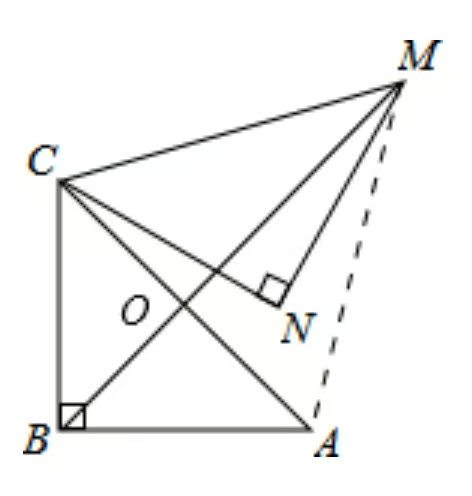
\includegraphics[width=0.25\linewidth]{figure/example_rotation1.jpg}
    
    \label{fig:enter-label}
\end{figure}
    
\end{example}



\chapter{圆}

\chapter{概率初步}

\chapter{反比例函数}

\chapter{相似}

\chapter{锐角三角函数}

\chapter{投影与视图}

\end{document}
